% Final project report - Mini-Lang compiler
% Build:  cd docs/report && xelatex report.tex && xelatex report.tex
% Each team member: edit the \fillin{...} fields (search for "fillin") and rebuild.
\documentclass[11pt,letterpaper]{article}

\usepackage{fontspec}
\setmainfont{TeX Gyre Pagella}
\setsansfont{Inter}
\setmonofont{DejaVu Sans Mono}[Scale=0.82]
\usepackage[margin=1in]{geometry}
\usepackage{microtype}
\usepackage{xcolor}
\usepackage{graphicx}
\usepackage{booktabs}
\usepackage{tabularx}
\usepackage{longtable}
\usepackage{array}
\usepackage{enumitem}
\usepackage{float}
\usepackage{caption}
\usepackage{titlesec}
\usepackage{fancyhdr}
\usepackage{listings}
\usepackage{fancyvrb}
\fvset{frame=single, framerule=0.4pt, rulecolor=\color{black!15}, fontsize=\small, xleftmargin=6pt, framesep=5pt}
\usepackage[hidelinks]{hyperref}

% ------------------------------------------------------------------ style
\definecolor{accent}{HTML}{1F4E8C}
\definecolor{codebg}{HTML}{F6F8FA}
\definecolor{fill}{HTML}{C0392B}
\newcommand{\fillin}[1]{\textcolor{fill}{\textbf{[#1]}}}   % fields to complete
\newcommand{\code}[1]{\texttt{#1}}

\titleformat{\section}{\sffamily\Large\bfseries\color{accent}}{\thesection.}{0.6em}{}
\titleformat{\subsection}{\sffamily\large\bfseries}{\thesubsection}{0.6em}{}
\titleformat{\subsubsection}{\sffamily\normalsize\bfseries}{}{0em}{}
\titlespacing*{\section}{0pt}{1.4em}{0.6em}
\titlespacing*{\subsection}{0pt}{1.1em}{0.4em}
\setlist{itemsep=2pt, topsep=4pt}
\captionsetup{font=small, labelfont=bf}
\setlength{\parskip}{0.45em}
\setlength{\parindent}{0pt}
\renewcommand{\arraystretch}{1.18}

\lstset{
  basicstyle=\ttfamily\small, backgroundcolor=\color{codebg},
  frame=single, rulecolor=\color{black!12}, framesep=4pt, xleftmargin=6pt, xrightmargin=6pt,
  columns=fullflexible, keepspaces=true, showstringspaces=false,
  aboveskip=0.6em, belowskip=0.6em, breaklines=true,
  commentstyle=\color{black!55}, keywordstyle=\color{accent}\bfseries,
}
\lstdefinelanguage{minilang}{morekeywords={int,bool,if,else,while,print,true,false},
  morecomment=[l]{//}, morecomment=[s]{/*}{*/}}
\lstdefinelanguage{tac}{morekeywords={goto,if,ifFalse,print}, morecomment=[l]{\#}}

\pagestyle{fancy}
\fancyhf{}
\fancyhead[L]{\sffamily\footnotesize Mini-Lang Compiler -- Final Project Report}
\fancyhead[R]{\sffamily\footnotesize Theory of Computation, UDLAP}
\fancyfoot[C]{\sffamily\footnotesize \thepage}
\renewcommand{\headrulewidth}{0.3pt}

\begin{document}

% ================================================================== TITLE PAGE
\begin{titlepage}
\centering
\vspace*{1.2cm}
{\sffamily\small UNIVERSIDAD DE LAS AMÉRICAS PUEBLA\\ School of Engineering\par}
\vspace{2.2cm}
{\sffamily\color{accent}\Huge\bfseries From Source to Execution:\\[0.25em] A Complete Mini-Lang Compiler\par}
\vspace{0.8cm}
{\Large Final Project Report\par}
\vspace{2cm}
\begin{tabular}{rl}
\textbf{Course:} & Theory of Computation \\
\textbf{Instructor:} & \fillin{Instructor name} \\[0.6em]
\textbf{Team members:} & Aldo André García Buenrostro (ID 185474) \\
 & \fillin{Team member 2 -- student ID} \\
 & \fillin{Team member 3 -- student ID} \\
 & \fillin{Team member 4 -- student ID} \\[0.6em]
\textbf{Date:} & \fillin{Submission date}, 2026 \\
\textbf{Repository:} & \fillin{https://github.com/USER/mini-lang-compiler} \\
\textbf{Release tag:} & \code{v1.0} \\
\end{tabular}
\vfill
{\small Language: Python 3 \quad$\cdot$\quad Target: Three-Address Code (TAC) + TAC interpreter\par}
\end{titlepage}

\setcounter{tocdepth}{1}
\tableofcontents
\newpage

% ================================================================== 1
\section{Executive Summary}

We built a complete compiler for \textbf{Mini-Lang}, a small statically typed imperative language with \code{int} and \code{bool} variables, arithmetic, relational and logical expressions, \code{if}/\code{else}, \code{while} and \code{print}. The compiler is written in Python~3 using only the standard library. It runs a five-phase pipeline (regex-based scanner, recursive-descent LL(1) parser, semantic analyzer, Three-Address Code generator and TAC interpreter) and translates a \code{.src} file into a \code{.tac} file, which it then executes. Running it takes two commands and no installation: \code{python scripts/compile.py prog.src -o prog.tac} and \code{python scripts/run.py prog.tac}. Alternatively, \code{python scripts/minilangc.py prog.src} runs every phase and writes every intermediate artifact.

\textbf{Evidence of correctness.}
\begin{itemize}
  \item \textbf{16/16 end-to-end tests pass.} The suite has 4 basic, 4 control-flow, 2 semantic-error and 2 integration programs, plus 4 extra negative tests, for \textbf{6 negative tests} in total. Each test is compared against expected TAC and expected output whose values were worked out by hand.
  \item \textbf{38/38 unit tests pass}, organized as one test class per phase.
  \item The grammar is mechanically verified to be \textbf{LL(1)}: 31 non-terminals, 59 productions and no conflicts.
\end{itemize}

\textbf{Key artifacts.}
\begin{itemize}
  \item \code{README.md}: build and run instructions, module overview, instruction set and worked examples.
  \item \code{docs/language-spec.md}: tokens, grammar, typing rules and semantics.
  \item \code{docs/grammar.txt} and \code{docs/design-diagram.png}.
  \item \code{tests/} (programs, expected files and unit tests).
  \item \code{scripts/}: \code{compile}, \code{run}, \code{minilangc}, \code{run\_tests} and \code{ll1\_check}.
  \item \code{.github/workflows/ci.yml}.
\end{itemize}

\subsection*{Deliverables and their mapping to the rubric (ABET SO1)}
\begin{tabularx}{\linewidth}{>{\raggedright}p{3.3cm} X}
\toprule
\textbf{Deliverable} & \textbf{Rubric criteria it evidences} \\
\midrule
Source code (\code{src/}) & \emph{Formulate}: each phase implements a formal model (regular expressions, LL(1) CFG, type rules, TAC). \emph{Apply}: modular Python design with tight interfaces. \\
README & \emph{Apply}: tooling and CLI usage. \emph{Formulate}: instruction set and translation scheme. \\
Language specification & \emph{Identify}: scope and non-goals. \emph{Formulate}: tokens, grammar and inference rules. \\
Test suite (16 + 38) & \emph{Evaluate}: positive, negative and run-time cases compared automatically against reviewed expected files. \\
Flow diagram & \emph{Formulate}: architecture and the artifacts each phase exchanges. \\
CI, Makefile, scripts & \emph{Apply}: reproducible, automated verification with modern tools. \\
Presentation & \emph{Evaluate} and \emph{Apply}: live evidence of correctness and of the diagnostics. \\
\bottomrule
\end{tabularx}

% ================================================================== 2
\section{Problem Framing \& Scope Control \textmd{(Identify)}}

A compiler is a typical \emph{complex engineering problem} in the sense of the rubric:
\begin{itemize}
  \item It has many interacting sub-problems (characteristic 5): five phases, each with its own formal model.
  \item Its technical requirements conflict (characteristic 1). Error recovery competes with simplicity, short-circuit semantics with straightforward code generation, and helpful diagnostics with failing fast.
  \item It has no single obvious solution (characteristic 2). The choice of parsing method, IR form, scoping model and run-time design each changes the rest of the pipeline.
\end{itemize}
Our first task was to fix the scope tightly enough that every feature in it could be finished and tested end to end.

\subsection{Language scope (in scope)}
\begin{itemize}
  \item \textbf{Types:} \code{int} (integers without overflow) and \code{bool}. There are no implicit conversions between them.
  \item \textbf{Declarations:} \code{int x; bool ok;} Each variable starts with a default value (\code{0} or \code{false}).
  \item \textbf{Assignments:} \code{x = e;}
  \item \textbf{Expressions:}
  \begin{itemize}
    \item arithmetic: \code{+ - * / \%}
    \item relational: \code{< <= > >= == !=}
    \item logical: \code{\&\& || !} (with short-circuit evaluation)
    \item unary minus and parentheses
  \end{itemize}
  \item \textbf{Control flow:} \code{if}/\code{else} (including \code{else if} chains) and \code{while}. The body of each is a block, and every block opens a new scope.
  \item \textbf{Output:} \code{print(e);} prints integers and booleans.
  \item \textbf{Comments:} \code{//} and \code{/* */}.
\end{itemize}

\subsection{Non-goals}
\begin{itemize}
  \item Optimizations such as SSA, register allocation and constant folding.
  \item Functions, arrays, strings, floating point and input.
  \item Object-oriented features, exceptions and threads.
  \item Multiple source files and declaration initializers (\code{int x = 1;}).
\end{itemize}
These exclusions are deliberate. They follow the project statement's ``out of scope'' list and keep the effort on correctness and integration.

\subsection{Constraints and assumptions}
\begin{itemize}
  \item \textbf{Platform:} any OS with Python $\geq$ 3.9. There are no third-party dependencies, so the project runs on a lab machine without a build step.
  \item \textbf{Frozen grammar subset:} the grammar in \code{docs/grammar.txt} was frozen at v1.0. Every change to it must keep \code{ll1\_check.py} free of conflicts.
  \item \textbf{Deterministic programs:} Mini-Lang has no input statement, so each test program has exactly one correct output.
\end{itemize}

\subsection{Risks and mitigations}
\begin{tabularx}{\linewidth}{>{\raggedright}p{4.2cm} X}
\toprule
\textbf{Risk} & \textbf{Mitigation} \\
\midrule
Token drift: scanner token kinds diverge from what the grammar and parser expect &
The scanner exports one list of token kinds (\code{TOKEN\_KINDS}), and the parser only references those names. Unit tests pin the kind of every operator and keyword, and the longest-match ordering. \\
Semantic corner cases: shadowing, out-of-scope use, cascading errors &
A scope stack with unique storage names for shadowed variables. A failed sub-expression has type \code{None}, which suppresses follow-up errors. Each case has a dedicated test. \\
Language semantics diverging from the host language: Python floors \code{-7 // 2} to $-4$, while C gives $-3$ &
Truncating division and modulo are implemented explicitly in the VM (\code{c\_div}, \code{c\_mod}) and covered by test \code{b03}. \\
Short-circuit semantics lost in TAC &
\code{\&\&} and \code{||} compile into jumps, not into a binary instruction. Test \code{c04} guards a division by zero behind \code{\&\&}. \\
Name clashes between user variables and temporaries (a user variable called \code{t1}) &
Names matching \code{t<N>} are reserved. A user variable \code{t1} is stored as \code{t1\_1}. There is a unit test for this. \\
Non-terminating test programs hang CI &
The VM has a step limit (default $10^6$) and reports a probable infinite loop. There is a unit test for this. \\
\bottomrule
\end{tabularx}

% ================================================================== 3
\section{Solution Design \& Justification \textmd{(Formulate)}}

\subsection{Architecture overview}
Figure~\ref{fig:pipeline} shows the pipeline. Every phase is a pure function from the previous phase's artifact to its own. Phases share only plain data (token lists and dictionaries), so every intermediate result can be serialized to JSON, inspected and tested on its own. The driver (\code{src/driver/pipeline.py}) runs the phases in order and \emph{fails fast}: phase $n+1$ runs only if phase $n$ reported no errors.

\begin{figure}[H]
\centering
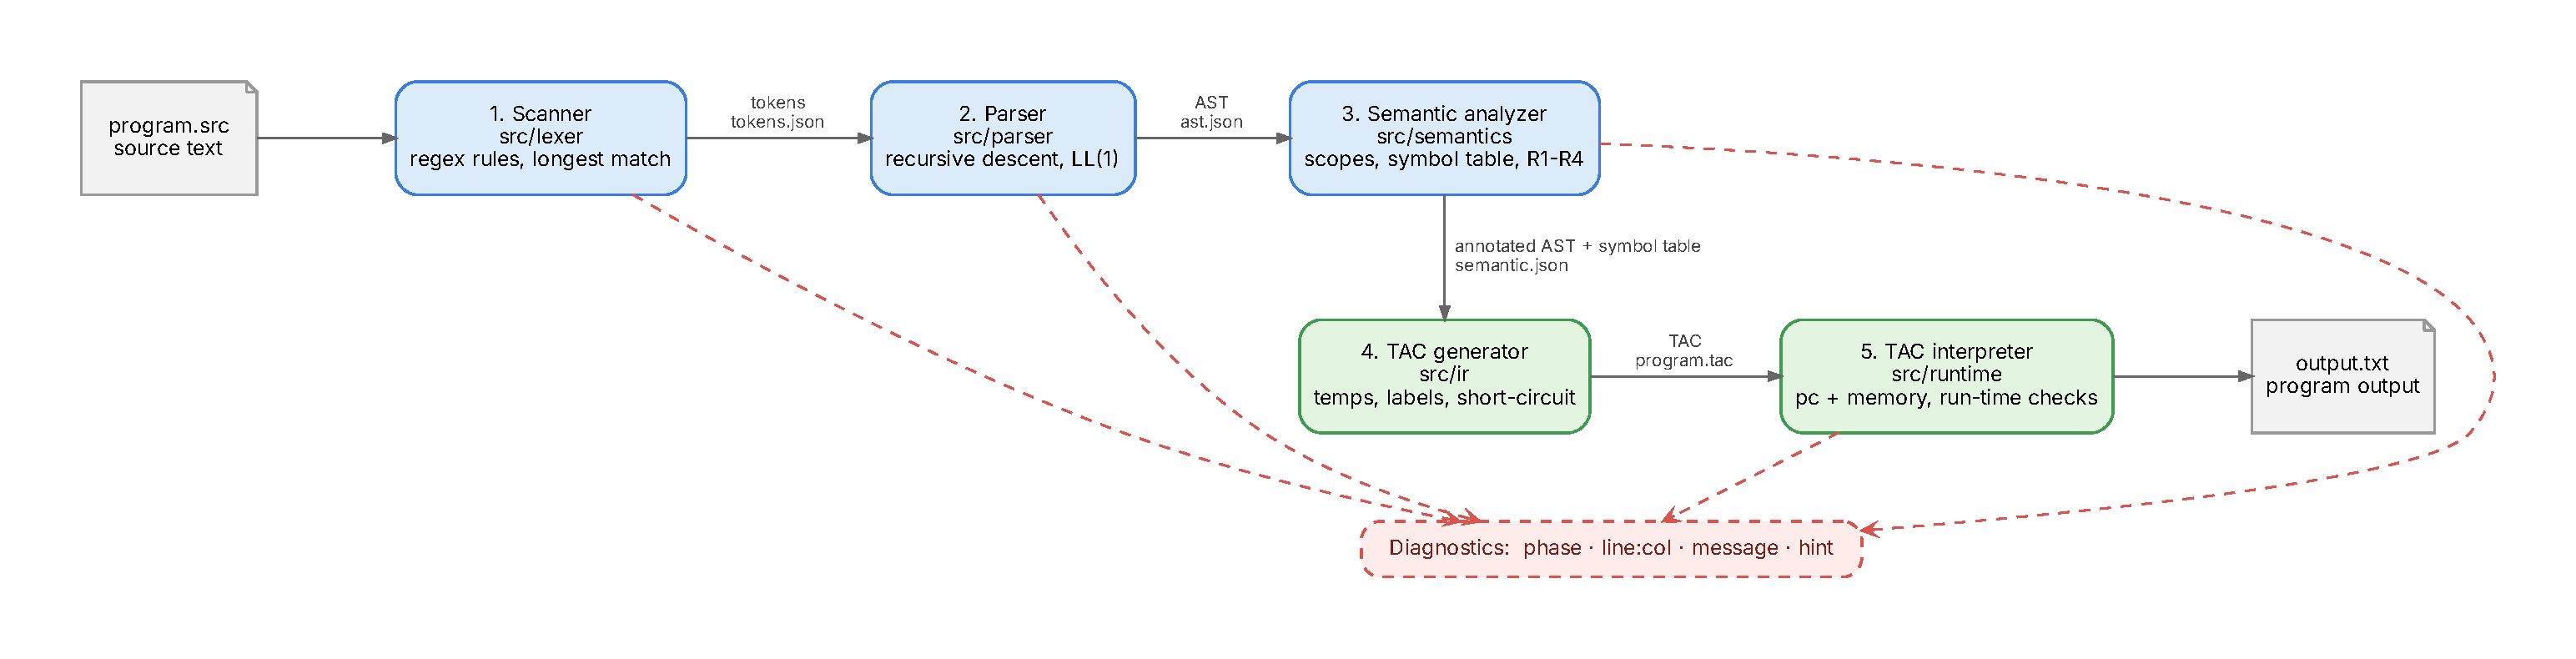
\includegraphics[width=\linewidth]{figures/pipeline-report.pdf}
\caption{Compiler pipeline, with the artifact produced by each phase. Every phase reports errors through one shared \code{Diagnostic} type.}
\label{fig:pipeline}
\end{figure}

\subsection{Module interfaces}

\begin{tabularx}{\linewidth}{>{\raggedright}p{2.6cm} >{\raggedright}p{4.6cm} X}
\toprule
\textbf{Phase} & \textbf{Entry point} & \textbf{Contract} \\
\midrule
Scanner & \code{scan(text)} & \code{str} $\rightarrow$ (\code{list[Token]}, \code{list[Diagnostic]}). A \code{Token} has \code{kind}, \code{lexeme}, \code{line} and \code{column}. \\
Parser & \code{parse(tokens)} & tokens $\rightarrow$ (AST, diagnostics). The fields of each node kind are listed in \code{ast\_nodes.py}. \\
Semantics & \code{analyze(ast)} & AST $\rightarrow$ \{status, summary, symbol\_table, errors, warnings, annotated\_ast\}. \\
Codegen & \code{generate(ast)} & annotated AST $\rightarrow$ \code{list[str]} of TAC lines. \\
Runtime & \code{TACMachine.run(text)} & TAC text $\rightarrow$ output lines; raises \code{TACRuntimeError}. \\
\bottomrule
\end{tabularx}

\textbf{Token kinds.} The scanner produces these kinds:
\begin{itemize}
  \item keywords: \code{INT BOOL IF ELSE WHILE PRINT TRUE FALSE}
  \item \code{IDENTIFIER} and \code{NUMBER}
  \item arithmetic operators: \code{PLUS MINUS STAR SLASH PERCENT}
  \item relational operators: \code{LESS LESS\_EQUAL GREATER GREATER\_EQUAL EQUAL NOT\_EQUAL}
  \item logical operators: \code{AND OR NOT}
  \item \code{ASSIGN}
  \item delimiters: \code{LPAREN RPAREN LBRACE RBRACE SEMICOLON COMMA}
  \item \code{EOF}
\end{itemize}

\textbf{AST snippet} for \code{x = 1;}. The semantic phase later adds \code{type} and \code{storage}.
\begin{lstlisting}
{"node": "Assignment", "target": "x",
 "value": {"node": "IntegerLiteral", "value": 1, "line": 5, "column": 5},
 "line": 5, "column": 1}
\end{lstlisting}

\textbf{Symbol table view}, an excerpt from \code{semantic.json} for the sample program:
\begin{center}\small
\begin{tabular}{llcllc}
\toprule
\textbf{name} & \textbf{type} & \textbf{scope} & \textbf{storage} & \textbf{declared} & \textbf{used} \\
\midrule
\code{x} & int & 0 & \code{x} & 1:1 & yes \\
\code{sum} & int & 0 & \code{sum} & 2:1 & yes \\
\code{ok} & bool & 0 & \code{ok} & 3:1 & yes \\
\bottomrule
\end{tabular}
\end{center}

\textbf{IR specification.} Table~\ref{tab:tac} lists the complete TAC instruction set. Operands are variables, temporaries (\code{t1, t2, \ldots}), integer literals, \code{true} and \code{false}.

\begin{table}[H]
\centering\small
\begin{tabularx}{0.92\linewidth}{>{\ttfamily}l X}
\toprule
\textrm{\textbf{Instruction}} & \textbf{Semantics} \\
\midrule
x := y & copy \\
x := op y & unary: \code{-} (negate), \code{!} (not) \\
x := y op z & binary: \code{+ - * / \% < <= > >= == !=} \\
goto L & unconditional jump \\
if y goto L & jump when \code{y} is true \\
if y relop z goto L & jump when the comparison holds (comparison folded into the jump) \\
ifFalse y [relop z] goto L & jump when false \\
print y & append the value of \code{y} to the output \\
L: & label (a jump target) \\
\bottomrule
\end{tabularx}
\caption{TAC instruction set.}
\label{tab:tac}
\end{table}

\subsection{Design choices and trade-offs}

\subsubsection*{Parsing method: hand-written recursive descent over an LL(1) grammar}
Two alternatives were considered. A parser generator such as PLY or ANTLR would hide the grammar behind a tool. A table-driven LR parser would make error messages harder to write. We wrote the grammar without left recursion and left-factored it, so each non-terminal maps directly to one method. This choice has three benefits:
\begin{enumerate}
  \item The code mirrors the theory taught in the course.
  \item \code{ll1\_check.py} can prove the grammar is LL(1) by computing FIRST and FOLLOW sets and the predictive table, so one token of lookahead is always enough.
  \item Panic-mode error recovery is straightforward to add.
\end{enumerate}
Operator precedence is encoded in the chain of non-terminals \code{or\_expr} $<$ \code{and\_expr} $<$ \ldots $<$ \code{unary}. Left associativity comes from building the tree left to right while consuming each \code{*\_tail} production.

\subsubsection*{TAC vs.\ bytecode}
We chose TAC for three reasons:
\begin{enumerate}
  \item The project statement requires it.
  \item TAC is human-readable, so the expected files in the test suite can be reviewed line by line and diffed in Git. Stack bytecode would have to be disassembled first.
  \item TAC keeps every intermediate result in a named temporary, which makes the correspondence between AST nodes and instructions explicit. That matters for an educational compiler.
\end{enumerate}
The cost is a less compact program and an interpreter that looks values up by name. Neither matters at this scale.

\subsubsection*{Control-flow representation}
Control flow uses symbolic labels and conditional and unconditional jumps. When a condition is a comparison, it is folded into the jump. This avoids a temporary and reproduces the project statement's example exactly (\code{if x < y goto L1}). \code{if}/\code{else} jumps to the \emph{then} branch and falls through into the \emph{else} branch, which is again the statement's layout. \code{while} tests at the top with \code{ifFalse}. To make the control flow visible, \code{ir/basic\_blocks.py} splits the TAC into basic blocks with the classic leader algorithm and builds the control-flow graph (Figure~\ref{fig:cfg}). The compiler writes this graph to \code{cfg.txt}.

\begin{figure}[H]
\centering
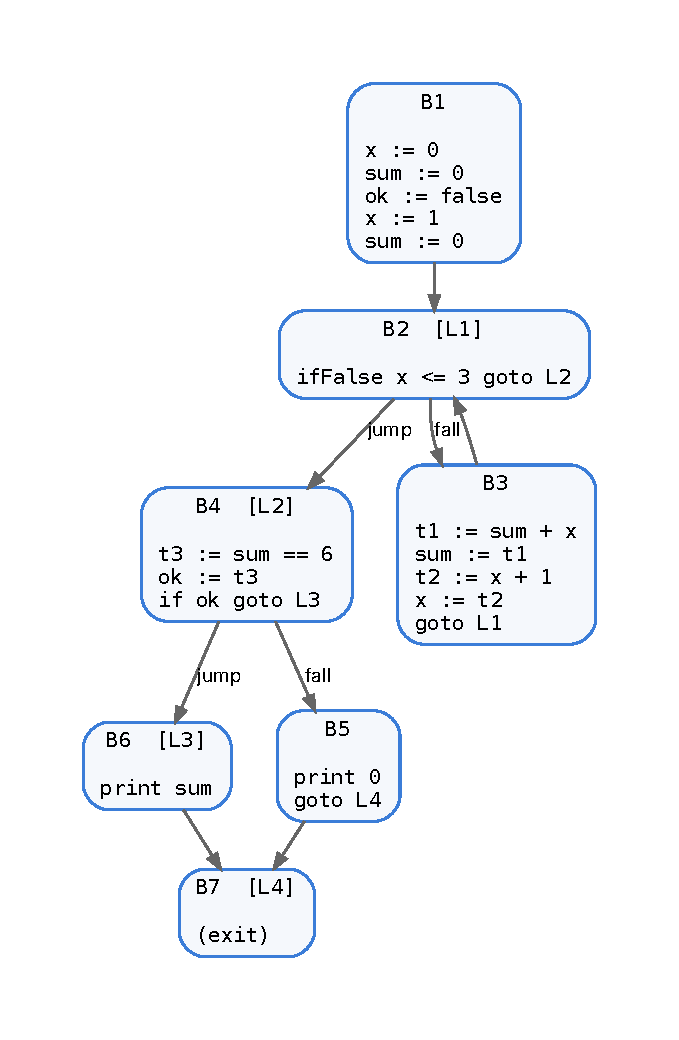
\includegraphics[height=8.6cm]{figures/cfg.pdf}
\caption{Basic blocks and CFG of the sample program. B2--B3 form the \code{while} loop; B4--B6 form the \code{if}/\code{else}.}
\label{fig:cfg}
\end{figure}

\subsubsection*{Type system and how it guides code generation}
The type system is static, has two types and allows no implicit conversions. The rules are given as inference rules in the language specification, §4. Type checking happens entirely before code generation, which gives the generator two guarantees:
\begin{itemize}
  \item It never checks types. Every operand already has the right type.
  \item Every variable reference carries a resolved \code{storage} name.
\end{itemize}
Shadowed variables get distinct storage names (\code{x}, \code{x\_1}, \ldots), so TAC can use a single flat namespace without scopes. Types also determine each declaration's default value (\code{0} or \code{false}) and how values print.

\subsubsection*{Error-handling strategy}
Every phase reports a \code{Diagnostic} with the phase, a 1-based \code{line:column}, a message and an optional hint. The CLI prints the offending source line with a caret under the column. The phases recover from errors differently:
\begin{itemize}
  \item The \textbf{scanner} skips the bad character and keeps scanning.
  \item The \textbf{parser} uses panic mode, synchronizing on \code{;}, \code{\}} or the start of a statement.
  \item The \textbf{semantic analyzer} keeps going after an error, and an undeclared operand does not produce a second type error.
\end{itemize}
So each phase reports \emph{all} of its errors in one run, and the pipeline then stops. Warnings (unused variable, use before assignment, shadowing, division by the constant 0) never stop compilation. At run time, the VM stops on the first error and reports the TAC line.

% ================================================================== 4
\section{Implementation Highlights}

\subsection{What we reused and what we implemented}
\begin{itemize}
  \item \textbf{Reused (Partial Exam 3):} the parser and the semantic analyzer. For the final project they were integrated with the scanner's token interface and moved to the shared \code{Diagnostic} type. They were also extended: the parser with \code{else if} and error recovery, the semantic analyzer with block scopes, storage names and warnings. \fillin{Adjust this paragraph to describe exactly what your team's Partial Exam 3 code contained.}
  \item \textbf{Implemented for this project:}
  \begin{itemize}
    \item the regex scanner with line and column tracking (\code{src/lexer})
    \item the TAC generator and the basic-block and CFG builder (\code{src/ir})
    \item the TAC interpreter (\code{src/runtime})
    \item the driver and CLIs (\code{src/driver}, \code{scripts/})
    \item the golden-test harness, the LL(1) checker and CI
  \end{itemize}
\end{itemize}
In total there are about 1,400 lines of compiler code and about 500 lines of tests and tooling.

\subsection{Key algorithms and patterns}
\begin{itemize}
  \item \textbf{Expression code generation:} a post-order walk of the expression tree. Each node returns the \emph{operand} that holds its value: a literal, a variable or a fresh temporary \code{tN}. A binary node emits \code{tN := a op b} once both operands are ready.
  \item \textbf{Short-circuit logic:} \code{a \&\& b} becomes \code{tN := a; ifFalse tN goto Lend; tN := b; Lend:}, and \code{||} is the same with \code{if}. The right operand is therefore never evaluated when the left one decides the result.
  \item \textbf{Branching and looping:} each construct allocates fresh labels from a counter. Because label names are unique, jumps can never cross between nested constructs.
  \item \textbf{Visitor dispatch:} the analyzer and the generator dispatch on \code{node["node"]} with \code{getattr(self, "gen\_" + kind)}, so adding a node kind means adding one method.
\end{itemize}

Listing~\ref{lst:codegen} shows the code-generation rules for conditions and \code{while} loops.
\begin{lstlisting}[language=Python, caption={Code generation for conditions and \code{while} loops (\code{src/ir/tac\_generator.py}).}, label=lst:codegen, morekeywords={def,return,if,in,self}]
def condition(self, node: dict) -> str:
    """Text placed between 'if'/'ifFalse' and 'goto'."""
    if node["node"] == "BinaryOp" and node["operator"] in COMPARISONS:
        left = self.expression(node["left"])     # fold the comparison
        right = self.expression(node["right"])   # into the jump itself
        return f"{left} {node['operator']} {right}"
    return self.expression(node)                 # any other bool operand

def gen_While(self, node):
    start, end = self.new_label(), self.new_label()
    self.place(start)                            # Lstart:
    cond = self.condition(node["condition"])     # re-evaluated every iteration
    self.emit(f"ifFalse {cond} goto {end}")      # exit when false
    self.statement(node["body"])
    self.emit(f"goto {start}")                   # back edge
    self.place(end)                              # Lend:
\end{lstlisting}

\subsection{Cross-module invariants}
\begin{enumerate}
  \item \textbf{Scanner $\rightarrow$ parser:} the token stream contains only kinds from \code{TOKEN\_KINDS}, and the parser appends exactly one \code{EOF} token.
  \item \textbf{Parser $\rightarrow$ semantics:} every AST node has \code{node}, \code{line} and \code{column}, plus exactly the fields listed for its kind in \code{ast\_nodes.py}.
  \item \textbf{Semantics $\rightarrow$ codegen:} if the status is \code{PASSED}, every expression has a \code{type}, and each \code{Declaration}, \code{Assignment} and \code{Identifier} has a \code{storage} name. Storage names are unique per symbol and never match \code{t<N>}.
  \item \textbf{Codegen $\rightarrow$ runtime:} every jump targets a label that the same program defines. The VM checks this at load time.
  \item \textbf{Fail fast:} a phase never runs on the output of a phase that reported errors.
\end{enumerate}

% ================================================================== 5
\section{Testing Strategy \& Result Interpretation \textmd{(Evaluate)}}

\subsection{Test plan}
\begin{itemize}
  \item \textbf{Unit tests} (\code{tests/unit}, 38 tests): one class per phase.
  \begin{itemize}
    \item scanner: keywords, longest match, positions, comments, lexical errors with hints
    \item parser: precedence, associativity, \code{else if}, recovery
    \item semantics: each rule R1--R4, operator typing, no cascading errors, scopes, storage names
    \item codegen: the exact TAC shapes from the project statement, short circuit, basic blocks
    \item runtime: C-style division, conditional jumps, undefined labels, unset variables, step limit
  \end{itemize}
  \item \textbf{End-to-end (golden) tests} (\code{tests/programs}, 16 programs): \code{run\_tests.py} compiles and runs each program and compares
  \begin{enumerate}
    \item the generated TAC with \code{tests/expected/<name>.tac}, and
    \item the program output, or the diagnostics for programs that must fail, with \code{<name>.out}.
  \end{enumerate}
  Every expected value was worked out by hand and is written as a comment next to the statement that produces it.
  \item \textbf{Negative tests:} programs that must fail in each phase (lexical, syntax, semantic and run time). They check that the failure happens \emph{in the right phase}, at the right \code{line:column}, with the right message.
  \item \textbf{Coverage goal:} every grammar production, every typing rule, every TAC instruction and every diagnostic category is exercised by at least one test.
\end{itemize}

\subsection{Test suite summary and pass/fail matrix}
\begin{longtable}{>{\ttfamily}l l l l c}
\toprule
\textrm{\textbf{Test}} & \textbf{Category} & \textbf{Expected result} & \textbf{Checked} & \textbf{Status} \\
\midrule
\endhead
b01\_declarations & basic & runs & TAC + output & PASS \\
b02\_assignments & basic & runs & TAC + output & PASS \\
b03\_arithmetic & basic & runs & TAC + output & PASS \\
b04\_relational\_logical & basic & runs & TAC + output & PASS \\
c01\_if\_else & control flow & runs & TAC + output & PASS \\
c02\_while & control flow & runs & TAC + output & PASS \\
c03\_nested & control flow & runs & TAC + output & PASS \\
c04\_short\_circuit & control flow & runs & TAC + output & PASS \\
s01\_undeclared & semantic error & fails in semantic & diagnostics & PASS \\
s02\_type\_error & semantic error & fails in semantic & diagnostics & PASS \\
i01\_primes & integration & runs & TAC + output & PASS \\
i02\_full\_program & integration & runs & TAC + output & PASS \\
x01\_lexical\_error & extra negative & fails in lexical & diagnostics & PASS \\
x02\_syntax\_error & extra negative & fails in syntax & diagnostics & PASS \\
x03\_duplicate\_declaration & extra negative & fails in semantic & diagnostics & PASS \\
x04\_runtime\_error & extra negative & fails at run time & TAC + output & PASS \\
\midrule
\multicolumn{5}{l}{\textbf{16/16 passed} (6 negative). Unit tests: \textbf{38/38 passed}. Grammar: LL(1), 0 conflicts.} \\
\bottomrule
\end{longtable}

\textbf{Failures and fixes.} All tests pass at \code{v1.0}. Three pitfalls each have a dedicated test, so a regression would show up as a failure:
\begin{itemize}
  \item Python's floor division would print $-4$ for \code{-7 / 2} (test \code{b03}).
  \item A user variable named \code{t1} would overwrite the temporary \code{t1} (unit test).
  \item An undeclared operand would also produce a spurious type error (unit test).
\end{itemize}
\fillin{Optional: add any real bugs your team found and fixed, with the commit that fixed each.}

\subsection{Representative transcript: short-circuit evaluation (test c04)}
\begin{lstlisting}[language=minilang]
d = 0;  n = 10;
ok = d != 0 && n / d > 1;      // right side must NOT be evaluated
print(ok);
\end{lstlisting}
Emitted TAC (excerpt of \code{tests/expected/c04\_short\_circuit.tac}):
\begin{lstlisting}[language=tac]
    t2 := d != 0
    t1 := t2
    ifFalse t1 goto L1          # d != 0 is false: skip n / d entirely
    t3 := n / d
    t4 := t3 > 1
    t1 := t4
L1:
    ok := t1
    print ok
\end{lstlisting}
\begin{center}\small
\begin{tabular}{lll}
\toprule
\textbf{Program} & \textbf{Expected output} & \textbf{Actual output} \\
\midrule
\code{c04\_short\_circuit} & \code{false true 0 4} & \code{false true 0 4} \\
\code{i01\_primes} & \code{2 3 5 7 11 13 17 19 23 29 10} & \code{2 3 5 7 11 13 17 19 23 29 10} \\
\code{i02\_full\_program} & \code{0 1 1 2 3 5 8 13 12 8 true 100 1} & identical \\
\bottomrule
\end{tabular}
\end{center}

\subsection{Representative transcript: semantic errors (test s02)}
\begin{lstlisting}
$ python scripts/compile.py tests/programs/s02_type_error.src
s02_type_error.src:4:1: semantic error: type mismatch: cannot assign a bool value to 'n' of type int
s02_type_error.src:5:1: semantic error: type mismatch: cannot assign an int value to 'b' of type bool
s02_type_error.src:6:7: semantic error: operator '*' expects int operands, but the left side is bool
s02_type_error.src:7:8: semantic error: while condition must be bool, but it is int
    while (n) {
           ^
    hint: use a comparison, e.g. (x != 0)
compilation failed in the semantic phase (4 error(s))
\end{lstlisting}

\subsection{Edge cases considered}
\begin{tabularx}{\linewidth}{>{\raggedright}p{3.8cm} X}
\toprule
\textbf{Edge case} & \textbf{Covered by} \\
\midrule
Precedence & \code{2+3*4=14}; \code{\&\&} binds tighter than \code{||}; \code{+} binds tighter than \code{==} (\code{b03}, \code{b04}, unit tests) \\
Associativity & \code{20-5-3=12}, \code{100/10/2=5}, i.e.\ left-associative (\code{b03}, unit test) \\
Negative arithmetic & \code{-7/2=-3}, \code{-7\%2=-1}, i.e.\ truncation as in C (\code{b03}) \\
Undeclared identifiers & never declared, and used after leaving the declaring block (\code{s01}) \\
Type mismatches & bool to int, int to bool, \code{bool * int}, \code{1 == true}, non-bool condition (\code{s02}, unit tests) \\
Scopes & shadowing three levels deep, with a different type in the inner scope (\code{i02}); duplicate in the same scope (\code{x03}) \\
Loops & a loop that never executes (\code{while (false)}), nested loops, compound conditions (\code{c02}--\code{c04}) \\
Run time & division by zero after partial output (\code{x04}); infinite loop stopped by the step limit (unit test) \\
\bottomrule
\end{tabularx}

\subsection{What the results mean}
\textbf{Confidence.} The end-to-end tests check the \emph{exact} TAC as well as the output, so they detect regressions in code shape as well as in behavior. For example, a change in label allocation or a lost short circuit would fail a test even if the printed output stayed the same. Because every phase has its own unit tests, a failure points to a single phase. We therefore have high confidence that the in-scope language is compiled correctly.

\textbf{Remaining risks and known limitations.}
\begin{itemize}
  \item The expected files were generated by the compiler and then reviewed against values computed by hand. A bug that produced plausible but wrong TAC with correct output could pass that review. The output check reduces this risk but does not remove it.
  \item Integers are unbounded, unlike C's fixed-width types.
  \item There is no input statement, no functions and no optimization of redundant copies (\code{t1 := t2}).
  \item Testing is example-based. There is no property-based or random program generation.
\end{itemize}

% ================================================================== 6
\section{Application of Tools \& Engineering Practice \textmd{(Apply resources)}}

\subsection{Tooling}
\begin{itemize}
  \item \textbf{Language and toolchain:} Python 3 (standard library only).
  \item \textbf{Diagrams:} Graphviz (\code{docs/design-diagram.dot} is rendered to SVG and PNG).
  \item \textbf{Report:} \LaTeX.
\end{itemize}
The CLI entry points in \code{scripts/} are:
\begin{itemize}
  \item \code{compile} and \code{run}, with the interface from the project statement;
  \item \code{minilangc}, which runs the full pipeline and writes every artifact;
  \item \code{run\_tests}, the golden-test harness, with \code{--update} and \code{--markdown};
  \item \code{ll1\_check}, which computes FIRST and FOLLOW and the predictive table.
\end{itemize}
The \code{Makefile} wraps these as \code{make test}, \code{make demo}, \code{make demo-error} and \code{make grammar}.

\subsection{Automation}
GitHub Actions (\code{.github/workflows/ci.yml}, also copied to \code{scripts/ci.yml}) runs four steps on every push, pull request and \code{v*} tag, on Python 3.9 and 3.12:
\begin{enumerate}
  \item unit tests
  \item end-to-end tests
  \item the LL(1) check of the grammar
  \item the demo pipeline
\end{enumerate}
The programs are deterministic, so no seeds are needed. Running \code{python scripts/run\_tests.py} reproduces every result in this report.

\subsection{Version control discipline}
\begin{itemize}
  \item \textbf{Branching model:} \code{main} always passes CI. Each component is developed on a feature branch (\code{feature/scanner}, \code{feature/codegen}, \code{feature/vm}, \code{feature/tests}, \code{docs/report}) and merged through a pull request reviewed by another team member.
  \item \textbf{Commits:} small and descriptive (e.g.\ ``codegen: fold comparisons into conditional jumps'').
  \item \textbf{Expected files:} changes to \code{tests/expected/} are committed only after reviewing \code{git diff}.
  \item \textbf{Release:} \code{v1.0} is the tagged release that this report describes.
\end{itemize}
\fillin{Insert links to notable PRs/commits and a screenshot of the commit graph.}

\subsection{Team process}
\begin{tabularx}{\linewidth}{>{\raggedright}p{3.2cm} >{\raggedright}p{4.4cm} X}
\toprule
\textbf{Role} & \textbf{Member} & \textbf{Responsibilities} \\
\midrule
Build / CI & \fillin{name} & scripts, Makefile, GitHub Actions, release tag \\
Runtime / VM & \fillin{name} & TAC interpreter, run-time diagnostics \\
Codegen & \fillin{name} & TAC generator, basic blocks, instruction-set documentation \\
Docs / Tests & \fillin{name} & test suite, expected files, README, language spec, report \\
\bottomrule
\end{tabularx}

The team held stand-ups twice a week and tracked work on an issue board with \emph{To do}, \emph{In progress}, \emph{Review} and \emph{Done} columns. \fillin{Insert issue-board snapshot.}

% ================================================================== 7
\section{Code Quality \& Documentation}

\subsection{Project layout and rationale}
\begin{lstlisting}
src/lexer/  src/parser/  src/semantics/  src/ir/  src/runtime/   one package per phase
src/common/      shared Diagnostic type          src/driver/   pipeline + CLIs
tests/programs/  *.src     tests/expected/  *.tac, *.out     tests/unit/   per-phase
docs/            README, language-spec.md, grammar.txt, design-diagram.{dot,svg,png}
scripts/         compile, run, minilangc, run_tests, ll1_check, ci.yml
\end{lstlisting}
The layout follows the structure recommended in the project statement. One package per phase means a package depends only on the phases before it and on \code{common}, never on later phases. This keeps the dependency graph acyclic and makes each phase testable on its own.

\subsection{Documentation assets}
\begin{itemize}
  \item \code{README.md}: quick start, CLI, artifacts, layout, interfaces, instruction set, three worked examples, error handling and limitations.
  \item \code{docs/language-spec.md}: tokens, the LL(1) grammar, precedence, typing rules as inference rules, dynamic semantics and the translation scheme.
  \item \code{tests/README.md}: the format of the expected files and the test inventory.
  \item Docstrings: every module begins with one describing its phase, and every grammar method is documented with the production it implements.
\end{itemize}

\subsection{Style and conventions}
\begin{itemize}
  \item PEP~8 naming and type hints on every public function.
  \item Pure functions as phase entry points; no global state.
  \item Error messages are lower-case and start with the phase.
  \item Comments explain \emph{why} rather than \emph{what} (see Listing~\ref{lst:codegen}).
\end{itemize}

\subsection{Maintainability: adding a \code{for} loop}
Adding \code{for (i = 0; i < n; i = i + 1) \{ \ldots \}} touches one place per phase:
\begin{enumerate}
  \item \textbf{Scanner:} add the keyword \code{"for": "FOR"}.
  \item \textbf{Grammar:} add the production \code{for\_stmt → for ( assign ; expression ; assign ) block}, where \code{assign} is an assignment without its \code{;}. Then re-run \code{ll1\_check.py}. \code{FOR} is a new first token, so no conflicts appear.
  \item \textbf{Parser:} add a \code{for\_statement} method and a \code{For} node to \code{ast\_nodes.py}.
  \item \textbf{Semantics:} add \code{visit\_For}, which reuses the R4 condition check.
  \item \textbf{Codegen:} add \code{gen\_For} as \emph{init}; \code{Lstart:}; \code{ifFalse c goto Lend}; \emph{body}; \emph{step}; \code{goto Lstart}; \code{Lend:}. The VM needs no change.
  \item \textbf{Tests:} add one control-flow program with its expected TAC and output.
\end{enumerate}

% ================================================================== 8
\section{Demonstration Plan (Presentation Readiness)}

\begin{tabularx}{\linewidth}{l >{\raggedright}p{2.8cm} X}
\toprule
\textbf{Time} & \textbf{Presenter} & \textbf{Content} \\
\midrule
0:00--1:30 & \fillin{name} & Language overview: features, non-goals, the pipeline diagram \\
1:30--3:00 & \fillin{name} & Design: LL(1) grammar check (\code{make grammar}), type rules, the TAC instruction set \\
3:00--5:30 & \fillin{name} & \textbf{Live demo 1 (valid):} \code{python scripts/minilangc.py tests/programs/i01\_primes.src}. Walk through \code{tokens.json}, \code{ast.txt}, \code{semantic.json}, \code{program.tac}, \code{cfg.txt} and the output. \\
5:30--7:00 & \fillin{name} & \textbf{Live demo 2 (semantic error):} \code{make demo-error}. Show the four diagnostics with line:column, caret and hint. Then fix one line and recompile. \\
7:00--8:30 & \fillin{name} & Evidence: \code{make test} (16/16 + 38/38); bugs avoided (C division, temp-name clash, cascading errors) \\
8:30--10:00 & all & Questions \\
\bottomrule
\end{tabularx}

\textbf{Failure demo.} If time allows, also run \code{x02\_syntax\_error} (three errors recovered in one run) and \code{x04\_runtime\_error} (output \code{10} followed by \code{runtime error: division by zero (TAC line 7)}). Together they show diagnostics in every phase.

% ================================================================== 9
\section{Reproducibility Appendix}

\textbf{Environment.}
\begin{itemize}
  \item Python $\geq$ 3.9, standard library only.
  \item Verified on Linux with Python 3.13. CI is configured for Python 3.9 and 3.12 on Ubuntu.
  \item Optional: \code{make} and Graphviz (only to re-render the diagram).
  \item \fillin{Add the OS and Python version of your own machine.}
\end{itemize}

\textbf{Build and run (copy and paste).}
\begin{lstlisting}
git clone https://github.com/USER/mini-lang-compiler.git
cd mini-lang-compiler && git checkout v1.0
python3 --version                                  # must be 3.9 or newer

python3 scripts/compile.py examples/pdf_example.src -o build/out.tac
python3 scripts/run.py build/out.tac               # prints 6
python3 scripts/minilangc.py examples/pdf_example.src -o build/demo

python3 -m unittest discover -s tests/unit -v      # 38 tests
python3 scripts/run_tests.py                       # 16/16 tests passed (6 negative tests)
python3 scripts/ll1_check.py docs/grammar.txt      # The grammar IS LL(1)
\end{lstlisting}

\textbf{Inputs and expected outputs.}
\begin{itemize}
  \item Test programs are in \code{tests/programs/*.src}.
  \item Expected TAC is in \code{tests/expected/*.tac}. The expected output or diagnostics are in the matching \code{*.out} file in the same folder.
  \item There are no \code{*.in} files because the language has no input.
  \item To diff a single test by hand:
\end{itemize}
\begin{lstlisting}
python3 scripts/compile.py tests/programs/c02_while.src -o build/c02.tac
diff build/c02.tac tests/expected/c02_while.tac
python3 scripts/run.py build/c02.tac | diff - tests/expected/c02_while.out
\end{lstlisting}

\textbf{Release tag:} \fillin{https://github.com/USER/mini-lang-compiler/releases/tag/v1.0}

% ================================================================== 10
\section{References}
\begin{enumerate}[label={[\arabic*]}]
  \item A.~V.~Aho, M.~S.~Lam, R.~Sethi, J.~D.~Ullman. \emph{Compilers: Principles, Techniques, and Tools}, 2nd ed. Addison-Wesley, 2006. Chapters 4 (LL(1) parsing, FIRST/FOLLOW), 6 (three-address code, short-circuit code) and 8.4 (basic blocks).
  \item R.~Nystrom. \emph{Crafting Interpreters}. Genever Benning, 2021. Recursive descent and panic-mode error recovery.
  \item M.~Sipser. \emph{Introduction to the Theory of Computation}, 3rd ed. Cengage, 2012. Regular and context-free languages.
  \item Course material, Theory of Computation, UDLAP: project statement and the compiler-pipeline slides.
\end{enumerate}

% ================================================================== 11
\section{Appendices}

\subsection*{A. Complete grammar (\code{docs/grammar.txt})}
\begin{Verbatim}
program     → stmt_list EOF
stmt_list   → stmt stmt_list | ε
stmt        → declaration | assignment | while_stmt | if_stmt | print_stmt | block
declaration → type IDENTIFIER ;              type      → int | bool
assignment  → IDENTIFIER = expression ;
while_stmt  → while ( expression ) block
if_stmt     → if ( expression ) block else_part
else_part   → else else_body | ε             else_body → block | if_stmt
print_stmt  → print ( expression ) ;
block       → { stmt_list }
expression  → or_expr
or_expr     → and_expr or_tail               or_tail   → || and_expr or_tail | ε
and_expr    → eq_expr and_tail               and_tail  → && eq_expr and_tail | ε
eq_expr     → rel_expr eq_tail               eq_tail   → eq_op rel_expr eq_tail | ε
eq_op       → == | !=
rel_expr    → add_expr rel_tail              rel_tail  → rel_op add_expr rel_tail | ε
rel_op      → < | <= | > | >=
add_expr    → mul_expr add_tail              add_tail  → add_op mul_expr add_tail | ε
add_op      → + | -
mul_expr    → unary mul_tail                 mul_tail  → mul_op unary mul_tail | ε
mul_op      → * | / | %
unary       → ! unary | - unary | primary
primary     → NUMBER | true | false | IDENTIFIER | ( expression )
\end{Verbatim}

\subsection*{B. Typing rules}
\begin{Verbatim}
Γ ⊢ n : int     Γ ⊢ true : bool     Γ ⊢ false : bool     Γ(x) = τ ⇒ Γ ⊢ x : τ
Γ ⊢ e1 : int,  Γ ⊢ e2 : int,  op ∈ {+,-,*,/,%}          ⇒ Γ ⊢ e1 op e2 : int
Γ ⊢ e1 : int,  Γ ⊢ e2 : int,  op ∈ {<,<=,>,>=}          ⇒ Γ ⊢ e1 op e2 : bool
Γ ⊢ e1 : τ,    Γ ⊢ e2 : τ,    op ∈ {==,!=}              ⇒ Γ ⊢ e1 op e2 : bool
Γ ⊢ e1 : bool, Γ ⊢ e2 : bool, op ∈ {&&,||}              ⇒ Γ ⊢ e1 op e2 : bool
Γ ⊢ e : int ⇒ Γ ⊢ -e : int            Γ ⊢ e : bool ⇒ Γ ⊢ !e : bool
Γ(x) = τ, Γ ⊢ e : τ ⇒ x = e; ok        Γ ⊢ c : bool ⇒ if (c) … / while (c) … ok
\end{Verbatim}

\subsection*{C. Full trace of the sample program across phases}
\textbf{Source} (\code{examples/pdf\_example.src}): the \code{while} loop that sums $1+2+3$, followed by \code{if (ok)}.
\textbf{Phase 1:} 62 tokens; the first line is \code{INT int 1:1, IDENTIFIER x 1:5, SEMICOLON ; 1:6}.
\textbf{Phase 2:} a \code{Program} node with 8 statements: 3 \code{Declaration}, 2 \code{Assignment}, \code{While}, \code{Assignment} and \code{If}.
\textbf{Phase 3:} \code{SEMANTIC ANALYSIS: PASSED}; 3 symbols; 0 errors; 0 warnings.
\textbf{Phase 4:} the TAC below, 17 instructions in 7 basic blocks (Figure~\ref{fig:cfg}).
\textbf{Phase 5:} 28 steps; output \code{6}.
\begin{lstlisting}[language=tac]
    x := 0                      L1:                          L2:
    sum := 0                        ifFalse x <= 3 goto L2       t3 := sum == 6
    ok := false                     t1 := sum + x                ok := t3
    x := 1                          sum := t1                    if ok goto L3
    sum := 0                        t2 := x + 1                  print 0
                                    x := t2                      goto L4
                                    goto L1                  L3: print sum
                                                             L4:
\end{lstlisting}

\end{document}
